\documentclass[14pt,xcolor=pdftex,dvipsnames,table]{beamer}\usepackage[]{graphicx}\usepackage[]{color}
%% maxwidth is the original width if it is less than linewidth
%% otherwise use linewidth (to make sure the graphics do not exceed the margin)
\makeatletter
\def\maxwidth{ %
  \ifdim\Gin@nat@width>\linewidth
    \linewidth
  \else
    \Gin@nat@width
  \fi
}
\makeatother

\definecolor{fgcolor}{rgb}{0.345, 0.345, 0.345}
\newcommand{\hlnum}[1]{\textcolor[rgb]{0.686,0.059,0.569}{#1}}%
\newcommand{\hlstr}[1]{\textcolor[rgb]{0.192,0.494,0.8}{#1}}%
\newcommand{\hlcom}[1]{\textcolor[rgb]{0.678,0.584,0.686}{\textit{#1}}}%
\newcommand{\hlopt}[1]{\textcolor[rgb]{0,0,0}{#1}}%
\newcommand{\hlstd}[1]{\textcolor[rgb]{0.345,0.345,0.345}{#1}}%
\newcommand{\hlkwa}[1]{\textcolor[rgb]{0.161,0.373,0.58}{\textbf{#1}}}%
\newcommand{\hlkwb}[1]{\textcolor[rgb]{0.69,0.353,0.396}{#1}}%
\newcommand{\hlkwc}[1]{\textcolor[rgb]{0.333,0.667,0.333}{#1}}%
\newcommand{\hlkwd}[1]{\textcolor[rgb]{0.737,0.353,0.396}{\textbf{#1}}}%

\usepackage{framed}
\makeatletter
\newenvironment{kframe}{%
 \def\at@end@of@kframe{}%
 \ifinner\ifhmode%
  \def\at@end@of@kframe{\end{minipage}}%
  \begin{minipage}{\columnwidth}%
 \fi\fi%
 \def\FrameCommand##1{\hskip\@totalleftmargin \hskip-\fboxsep
 \colorbox{shadecolor}{##1}\hskip-\fboxsep
     % There is no \\@totalrightmargin, so:
     \hskip-\linewidth \hskip-\@totalleftmargin \hskip\columnwidth}%
 \MakeFramed {\advance\hsize-\width
   \@totalleftmargin\z@ \linewidth\hsize
   \@setminipage}}%
 {\par\unskip\endMakeFramed%
 \at@end@of@kframe}
\makeatother

\definecolor{shadecolor}{rgb}{.97, .97, .97}
\definecolor{messagecolor}{rgb}{0, 0, 0}
\definecolor{warningcolor}{rgb}{1, 0, 1}
\definecolor{errorcolor}{rgb}{1, 0, 0}
\newenvironment{knitrout}{}{} % an empty environment to be redefined in TeX

\usepackage{alltt}

% Specify theme
\usetheme{Madrid}
% See deic.uab.es/~iblanes/beamer_gallery/index_by_theme.html for other themes
\usepackage{caption}
\usepackage{tikz}
\usepackage{multirow}
% Specify base color
\usecolortheme[named=OliveGreen]{structure}
% See http://goo.gl/p0Phn for other colors

% Specify other colors and options as required
\setbeamercolor{alerted text}{fg=Maroon}
\setbeamertemplate{items}[square]

% Title and author information
\title{Economic Forecast}
\author{Rob Hayward}
\IfFileExists{upquote.sty}{\usepackage{upquote}}{}
\begin{document}

\begin{frame}
\titlepage
\end{frame}


\begin{frame}{Outline}
\tableofcontents
\end{frame}

\section{Introduction}
\begin{frame}{Aims}
The aim is to forecast interest rate changes. This will require
\pause
\begin{itemize}[<+-| alert@+>]
\item An understanding of the central bank
\item Some knowledge of the current state of the economy
\item A forecast of how the economy will evolve in the future
\item An assessment of what this means for monetary policy
\end{itemize}
\pause
Draw on what you learnt in EC271 and EC284
\end{frame}


\section{Central bank}
\begin{frame}{Central bank}
It is important to know central bank policy if you wnat to understand what they will do
\pause
\begin{itemize}[<+-| alert@+>]
\item How do they see the economy?
\item What is their main focus/concern?
\item Do they have a specific mandate? 
\item When do they meet?  How do they decide policy?  What is the nature of the usual policy change? 
\end{itemize}
\end{frame}


\section{Output gap}
\begin{frame}{Output gap}
\begin{knitrout}
\definecolor{shadecolor}{rgb}{0.969, 0.969, 0.969}\color{fgcolor}\begin{figure}[]

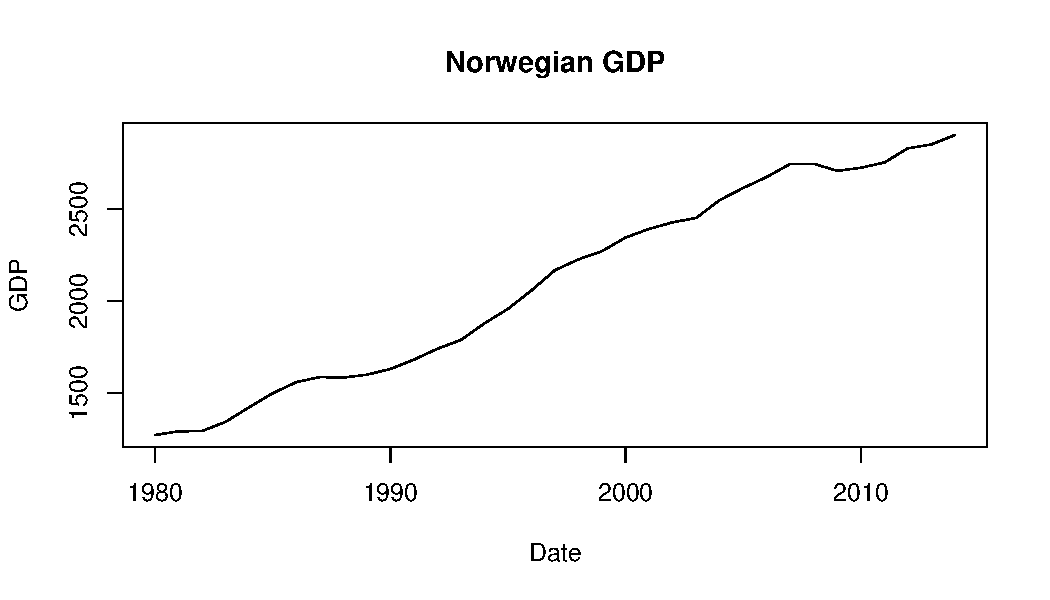
\includegraphics[width=\maxwidth]{figure/GDP-1} \caption[Norwegian real GDP]{Norwegian real GDP\label{fig:GDP}}
\end{figure}


\end{knitrout}
\end{frame}

\begin{frame}{Finding the trend}
There are five methods to find the trend
\pause
\begin{itemize}[<+-| alert@+>]
\item Estimation of a growth rate 
\item Linear trend
\item Quadratic tend
\item Hodrick-Prescott filter
\item Centered moving average
\end{itemize}
\end{frame}


\section{GDP components}
%\begin{frame}{GDP components}
%<<gdp, echo=FALSE, warning=FALSE, message=FALSE, fig.height=4>>=
%library(dplyr)
%library(tidyr)
%names  <- c("Country", "Currency", "Year", "Final_Consumption", "Consumption",
%            "Government", "GCF", "GFCF", "Inventories", "Exports", "Imports", %"GDP")
%da <- read.csv("../../ECM04/Financial_System/Data/UNGNP.csv")
%names(da) <- names
%head(da)
%da <- da[,-13]
%# Change the country for savings ratio
%unique(da$Country)
%da %>%
%  filter(Country == "Germany") %>%
%  select(Year, Consumption, Government, GFCF, Exports, Imports)%>%
%  head()%>%
%  barplot(main = "GDP")
%@
%\end{frame}
\section{Taylor rule}
\begin{frame}{Taylor rule}
Taylor rule 
\begin{block}{}
\begin{equation*}
i_t = \pi_t + r_t^* + \alpha_{\pi}(\pi_t - \pi_t^*) + \alpha_y(y_t - \bar{y}_t)
\end{equation*}
\end{block}
where $i_t$ is the nominl interest rate; $\pi_t$ is the inflation rate; $r_t^*$ is the real interest rate; $y_t$ is GDP; $\pi_t^*$ is the inflation target; $\bar{y}_t$ is the potential rate of GDP growth; $\alpha_{\pi}$ is the elasticity of interest rates to inflation; $\alpha_y$ is the elasticity of interest rates to the potential growth rate.  
\end{frame}

\begin{frame}{Estimation of rule}
\begin{itemize}[<+-| alert@+>]
\item Add other variables if appropriate (exchange rate)
\item OLS regression estimation of $\alpha_{\pi}$ and $\alpha_y$
\item What does the model say about interest rates?
\item What happens to inflation, GDP or the exchange rate from this point? 
\end{itemize}
\end{frame}



%[<+-| alert@+>]
\end{document}
